\chapter{Data set}
\label{ch:data_set}

\section{Data description}
%TODO change
The data set consists of spine-focused CT scans of 125 patients with varying types of pathologies. 

In the case of the detection model the dense labelling contains two values: 0 representing background and 1 representing vertebrae. 

The identification model’s dense labelling contains values from 0 to 26. Whilst 0 representing background, 1 representing C1 vertebrae up to 26 representing S2 vertebrae.

\begin{figure}[h]
    \centering 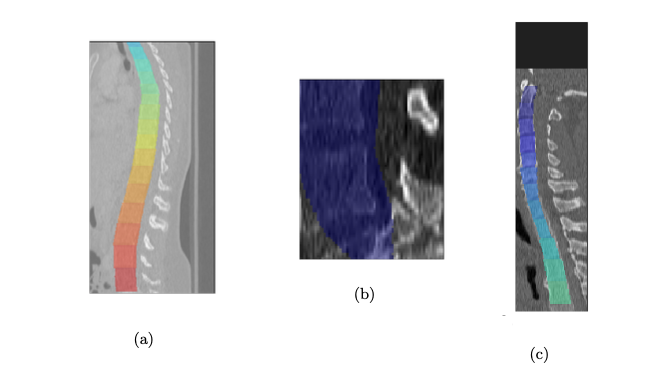
\includegraphics[width=9cm]{images/labeled_data.png}
    \caption {(a) shows a dense labelling, (b) shows an example of a sample used to train the detection model, (c) shows an example of a sample used to train the identification model. Note: The size of the sample is 8 x 80 x 320, if the original scan is not larger enough to fill those dimensions some padding is added, as can be seen at the top.}
    \label{fig:labeled_data}
\end{figure}

